\chapter{Результаты работы} \label{ch4}
Предлагается построить симуляцию на основании реально существующего участка дороги в г. Москве.
	
\section{Анализ входных данных} \label{ch4:sec1}
\subsection{Карта исследуемого участка дороги}
\begin{figure}[!htbp]
		\centering
		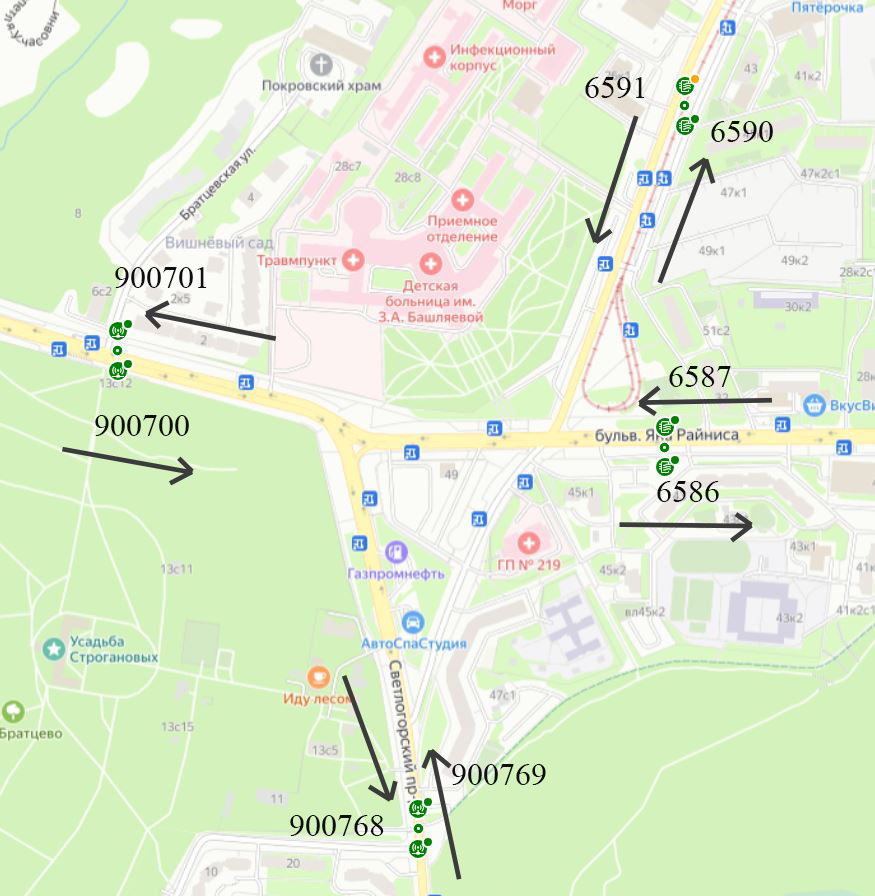
\includegraphics[height=0.5\textheight,valign=t]{my_folder/images//radiodetectors.JPG}
		
\captionsetup{justification=centering} %центрировать
	\caption{Участок дорожной карты с обозначением номеров радиодетекторов} 
\end{figure}

На \firef{fig:radiodetectors-map} номерами 1 и 2 обозначены светофорные объекты, регулирующие движение на представленных перекрестках.
\newpage
\begin{figure}[!htbp]
		\centering
		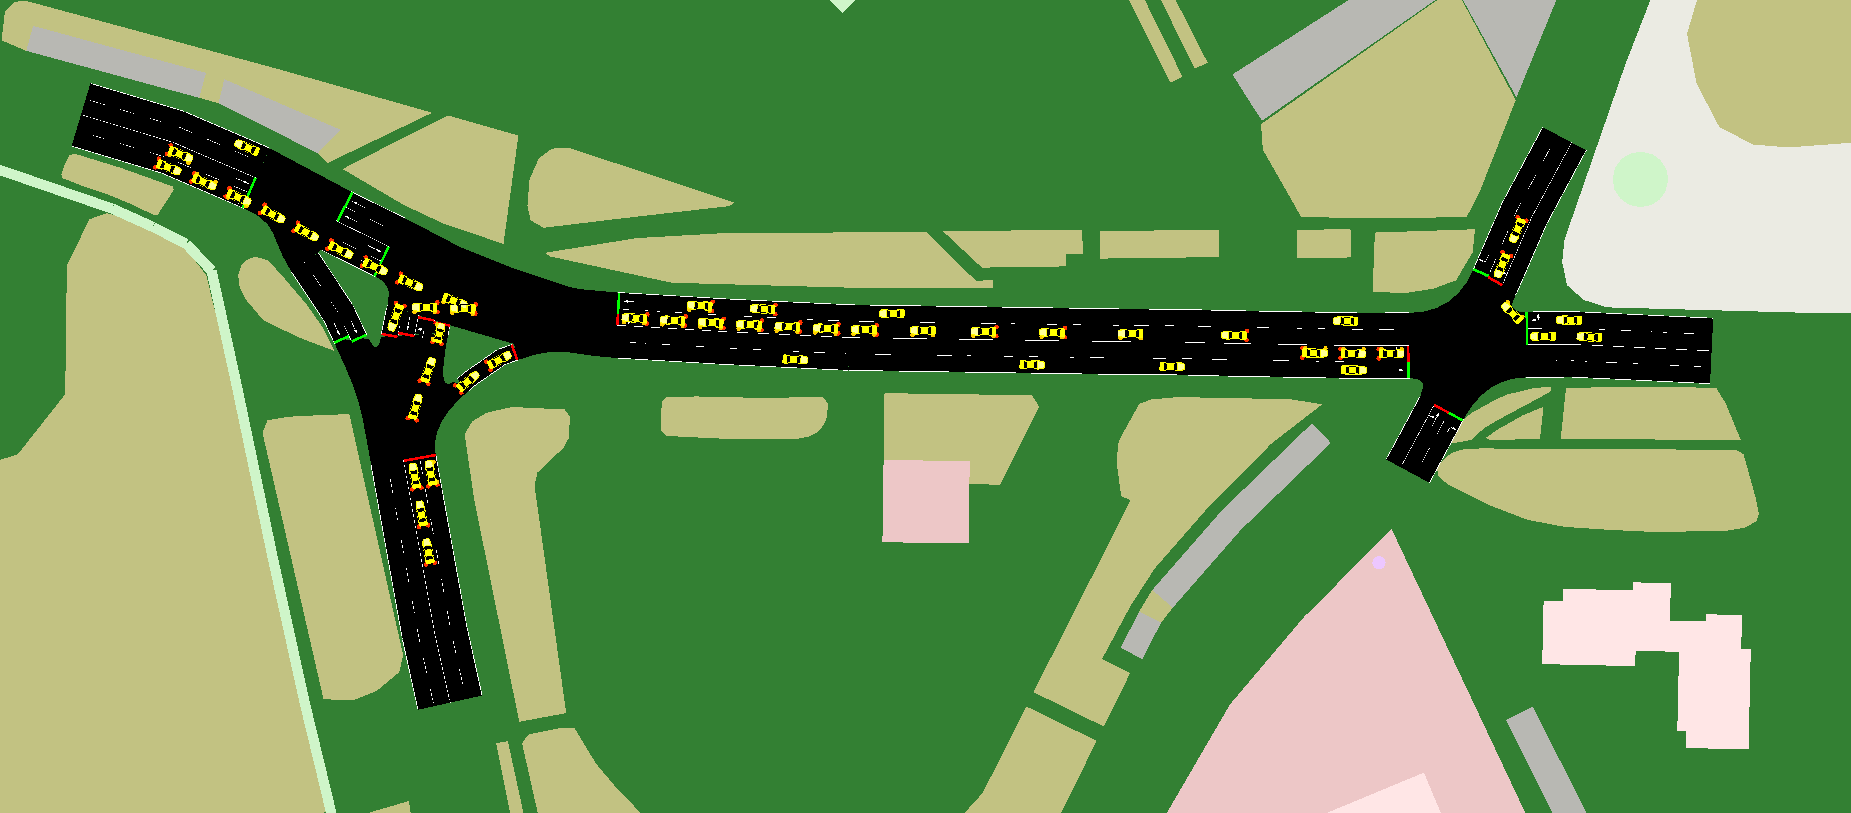
\includegraphics[height=0.3\textheight,valign=t]{my_folder/images//sumo-gui-roadmap.png}
		
\captionsetup{justification=centering} %центрировать
	\caption{Модель участка дороги на основе \firef{fig:radiodetectors-map}} 
\end{figure}


\begin{figure}[!htbp]
    \centering
    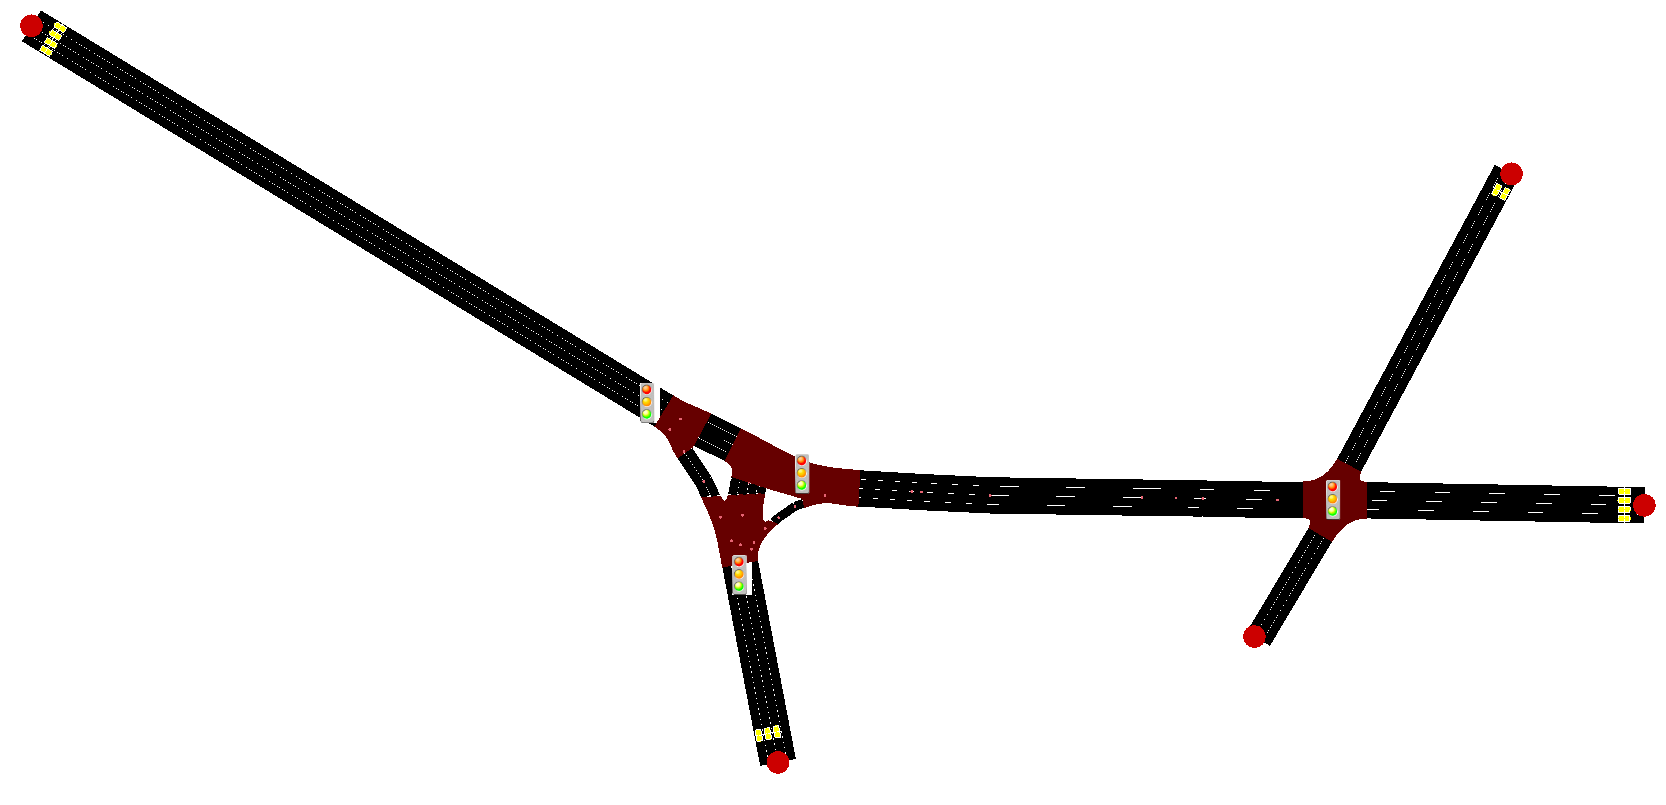
\includegraphics[height=0.2\textheight,valign=t]{my_folder/images//detectors-setting.png}
    
\captionsetup{justification=centering} %центрировать
\caption{Места расположения детекторов на карте}\label{fig:detectors-setting}
\end{figure}

\subsection{Определение состояний}
Информация о направлениях движения, регулируемых светофорными объектами 1 и 2, представлена в паспортах СО соответственно.
\begin{figure}[ht]
	\adjustbox{minipage=1.3em,valign=t}{\subcaption{}\label{fig:linked-phase-a}}%
	\begin{subfigure}[t]{\dimexpr.5\linewidth-1.3em\relax}
		\centering
		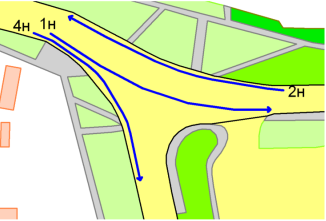
\includegraphics[width=.70\linewidth,valign=t]{my_folder/images/linked-0.png}
	\end{subfigure}
\hfill %выровнять по ширине
	\adjustbox{minipage=1.3em,valign=t}{\subcaption{}\label{fig:spbpu_sc-b}}%
	\begin{subfigure}[t]{\dimexpr.5\linewidth-1.3em\relax}
		\centering
		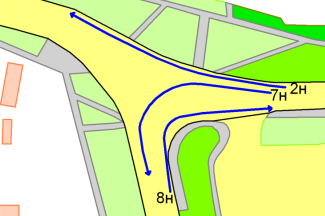
\includegraphics[width=.70\linewidth,valign=t]{my_folder/images/linked-1.png}
	\end{subfigure}
\\[20pt]
	\adjustbox{minipage=1.3em,valign=t}{\subcaption{}\label{fig:spbpu_sc-c}}%
\begin{subfigure}[t]{\dimexpr.5\linewidth-1.3em\relax}
	\centering
	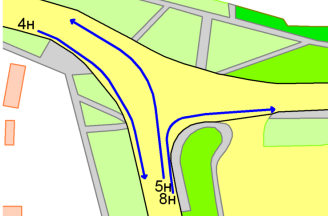
\includegraphics[width=.70\linewidth,valign=t]{my_folder/images/linked-2.png}
\end{subfigure}%
\hfill %выровнять по ширине
\adjustbox{minipage=1.3em,valign=t}{\subcaption{}\label{fig:spbpu_sc-d}}%
\begin{subfigure}[t]{\dimexpr.5\linewidth-1.3em\relax}
	\centering
	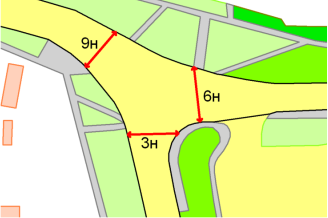
\includegraphics[width=.70\linewidth,valign=t]{my_folder/images/linked-red.png}
\end{subfigure}
\captionsetup{justification=centering} %центрировать
\caption{Направлениия движения СО 1} 
\label{fig:linked-phases}
\end{figure}

\clearpage
\begin{figure}[ht]
	\adjustbox{minipage=1.3em,valign=t}{\subcaption{}\label{fig:separate-phase-a}}%
	\begin{subfigure}[t]{\dimexpr.5\linewidth-1.3em\relax}
		\centering
		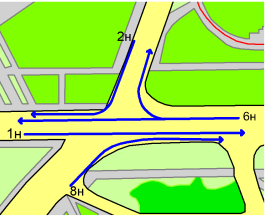
\includegraphics[width=.80\linewidth,valign=t]{my_folder/images/separate-0.png}
	\end{subfigure}
\hfill %выровнять по ширине
	\adjustbox{minipage=1.3em,valign=t}{\subcaption{}\label{fig:separate-phase-b}}%
	\begin{subfigure}[t]{\dimexpr.5\linewidth-1.3em\relax}
		\centering
		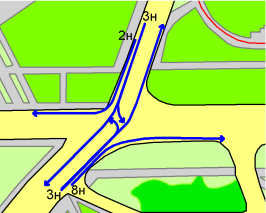
\includegraphics[width=.80\linewidth,valign=t]{my_folder/images/separate-1.png}
	\end{subfigure}
\\[20pt]
	\adjustbox{minipage=1.3em,valign=t}{\subcaption{}\label{fig:separate-phase-c}}%
\begin{subfigure}[t]{\dimexpr.5\linewidth-1.3em\relax}
	\centering
	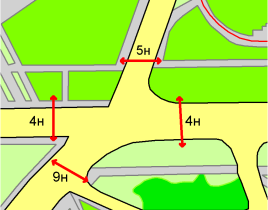
\includegraphics[width=.80\linewidth,valign=t]{my_folder/images/separate-red.png}
\end{subfigure}%
\hfill %выровнять по ширине
\adjustbox{minipage=1.3em,valign=t}{\subcaption{}\label{fig:separate-phase-d}}%
\begin{subfigure}[t]{\dimexpr.5\linewidth-1.3em\relax}
	\centering
	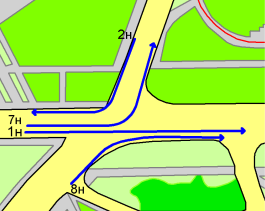
\includegraphics[width=.80\linewidth,valign=t]{my_folder/images/separate-2.png}
\end{subfigure}
\captionsetup{justification=centering} %центрировать
\caption{Направлениия движения СО 2} 
\label{fig:linked-phases}
\end{figure}

\clearpage
%\FloatBarrier % заставить рисунки и другие подвижные (float) элементы остановиться
\clearpage
\newpage

\subsection{Сводка данных о трафике}

\section{Выводы} \label{ch4:conclusion}

Текст выводов по главе \thechapter.

%% Вспомогательные команды - Additional commands
%
%\newpage % принудительное начало с новой страницы, использовать только в конце раздела
%\clearpage % осуществляется пакетом <<placeins>> в пределах секций
%\newpage\leavevmode\thispagestyle{empty}\newpage % 100 % начало новой страницы